\chapter{Metodologia}


\section{Distribuição Beta}

Segundo \cite{gomes2005} a distribuição beta é muito utilizada para modelar experimentos aleatórios cujas variáveis assumem valoreos no intervalo $(0,1)$, dada a grande flexibilidade de ajuste que seus parâmetros proporcionam. Uma variável aleatória contínua $Y$ tem distribuição beta com parâmetros $\alpha_1 > 0$ e $\alpha_2 > 0$ e sua função de densidade de probabilidade da forma

\begin{equation}
f(y)=\frac {\Gamma(\alpha_1+\alpha_2)}{\Gamma(\alpha_1)\Gamma(\alpha_2)} y^{\alpha_1-1}(1-y)^{\alpha_2-1}I_{(0,1)}(y)
\end{equation}

em que $\Gamma$ é uma função gama e $I$ representa a função indicadora.

Os parâmetros $\alpha_1$ e $\alpha_2$ são parâmetros de ajuste, por resultar em diferentes formas de densidade em $(0,1)$ através da escolha de $\alpha_1$ e $\alpha_2$. Geralmente quando $\alpha_1 = \alpha2$ as densidades são simétricas, assim, a distribuição beta pode ser vista como uma família de distribuições  \ref{fig06}.


\begin{figure}[!h]
	\centering
	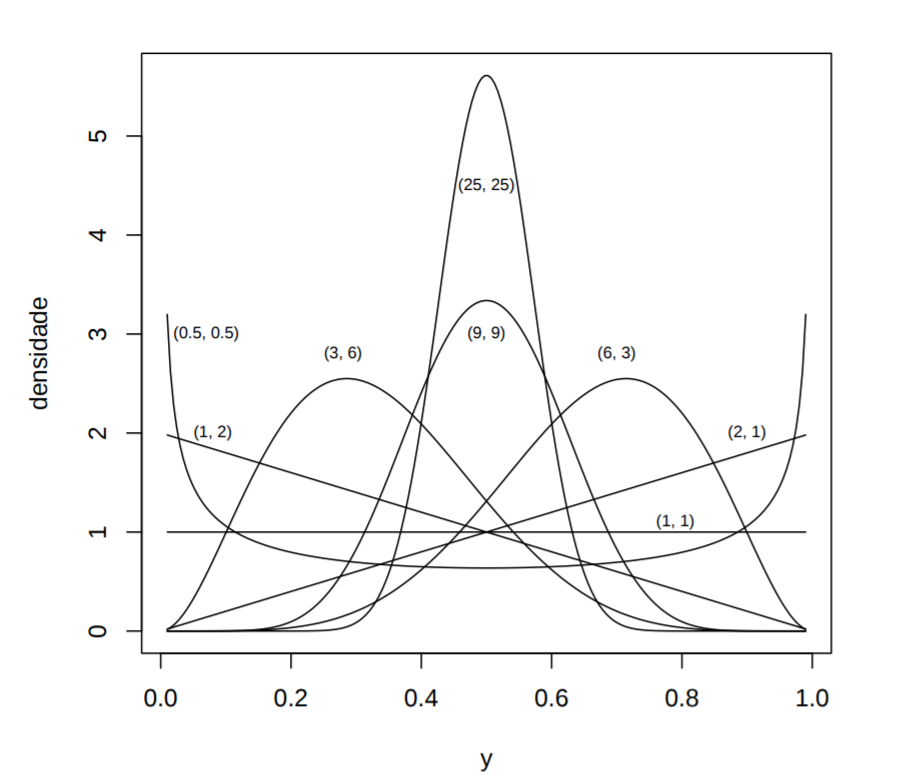
\includegraphics[keepaspectratio=true,scale=0.3]{figuras/dist-beta1.png}
	\caption{Gráfico de densidade beta para diferentes valores de $\alpha_1$ e $\alpha_2$}
	Fonte: \cite{gomes2005}
	\label{fig06}
\end{figure}


Ao se fixar $\alpha_2$, no lado esquerdo da \ref{fig07}, é obtido a variação de densidade beta para diferentes valores de $\alpha_1$; O mesmo acontece ao se fixar o $\alpha_1$, no lado direito da \ref{fig07}, é obtido a variação de densidade beta para diferentes valores de $\alpha_2$. Ao permutar $\alpha_1$ e $\alpha_2$ ocorre uma reflexão em torno da reta $y = 0,5$, devido à expressão da densidade como função de $y$ e $y-1$. 

Se $Y$ tem distribuição beta, a esperança é dada por

$$ E(Y) = \frac {\alpha_1}{\alpha_1 + \alpha_2} $$

e a variância é dada por

$$ Var(Y) = \frac{\alpha_1\alpha_2}{(\alpha_1+\alpha_2)^2(\alpha_1+\alpha_2+1)} $$


\begin{figure}[!h]
	\centering
	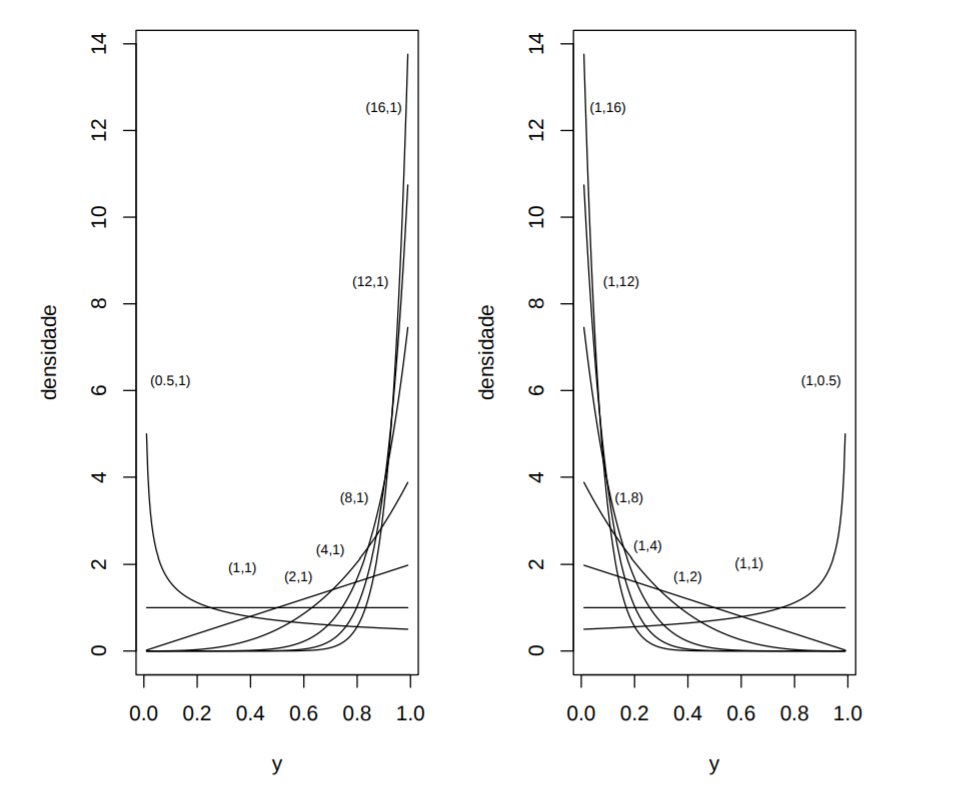
\includegraphics[keepaspectratio=true,scale=0.4]{figuras/dist-beta2.png}
	\caption{Gráfico de densidade beta para diferentes valores de $\alpha_1$ e $\alpha_2$, fixando $\alpha_2 = 1$ (esquerda) e $\alpha_1 = 1$ (direita)}
	Fonte: \cite{gomes2005}
	\label{fig07}
\end{figure}


Através da equação da variância pode-se observar que a variabilidade de $Y$ diminui à medida que se aumenta os valores dos dois parâmetro; pode ser visto na Figura \ref{fig06} quando as distribuições são simétricas.


\section{Distribuição Dirichlet}


Segundo \apud{lovelace1998}{barbosa2018} a distribuição de Dirichlet é uma família de distribuições de probabilidade multivariada contínuas, parametrizada por um vetor de parâmetros $\alpha$, denotada por $Dir(\alpha)$. É uma generalização multivariada da distribuição Beta, podendo ser empregada no estudo da distribuição de vetores aleatórios, cuja as variáveis aleatórias estejam compreendidas no intervalo (0,1) e a soma é igual a 1.

Seja $\textbf{p}$ um vetor aleatório cujos elementos somam 1, de modo que $p_{k}$ represente a proporção do item \textit{k}. De acordo \cite{minka2000}, sob o modelo de Dirichlet com o vetor de parâmetros $\alpha$, a densidade de probabilidade em $\textbf{p}$ é


\begin{equation}
p(\boldsymbol {p}) \sim \mathcal{D}(\alpha_{1},\dots,\alpha_{k}) = \frac {\Gamma(\sum_{k} \alpha_{k})}{\prod_{k}\Gamma(\alpha_{k})} \prod_{k} p_{k}^{\alpha_{k}-1}
\end{equation}


Onde $p_{k} > 0$ 
\begin{equation}
\sum_{k} p_{k} = 1
\end{equation}    

O parâmetro $\alpha$ é um vetor $k$ com componentes $\alpha_i > 0$, e onde $\Gamma(x)$ é a função Gamma \cite{blei2003}.
Os parâmetros $\alpha$ são estritamente positivos e um fato importante é que as densidades marginais da distribuição Dirichlet são beta \cite{gomes2005}.

Seja $\phi = \sum_{i=1}^{p} \alpha_i$


\begin{equation}
E(Y_i) = \frac{\alpha_i}{\phi}, \quad i = 1, \dots, p-1,
\end{equation} 

\begin{equation} \label{dir:var}
Var(Y_i) = \frac{\alpha_i(\phi-\alpha_i)}{\phi^2(\phi+1)}, \quad i = 1, \dots, p-1,
\end{equation} 



Segundo \cite{blei2003} uma variável aleatória Dirichlet $k$-dimensional $\theta$ pode assumir valores no $(k-1)$-simplex (um vetor-$k$ $\theta$ encontra-se no $(k-1)$-simplex se $\theta_i \geq 0$,
$\sum_{i=1}^{k} \theta_i =1)$. 
O Dirichlet é uma distribuição conveniente no simplex - está na família exponencial, tem estatísticas suficientes de dimensão finita e é conjugada à distribuição multinomial.


Para a maior compreensão da distribuição de Dirichlet, o trabalho de visualização foi replicado com base em \cite{liu2019}. Com $k=3$ e $2$-simplex, $k=(\alpha_1, \alpha_2, \alpha_3)$. 

Em distribuições simétricas para valores de $\alpha<1$, a distruibuição se concentra nos cantos e ao longo dos limites do simplex. No caso de $\alpha=1$, $k=(1,1,1)$, produz uma distribuição uniforme, onde todos os pontos do simplex são igualmente prováveis. Para valores $\alpha>1$, a distribuição tende para o centro do simplex, como pode ser visto na \ref{fig08}. Conforme $\alpha_i$ aumenta, a distribuição se torna mais concentrada em torno do centro do simplex. 


\begin{figure}[!h]
	\centering
	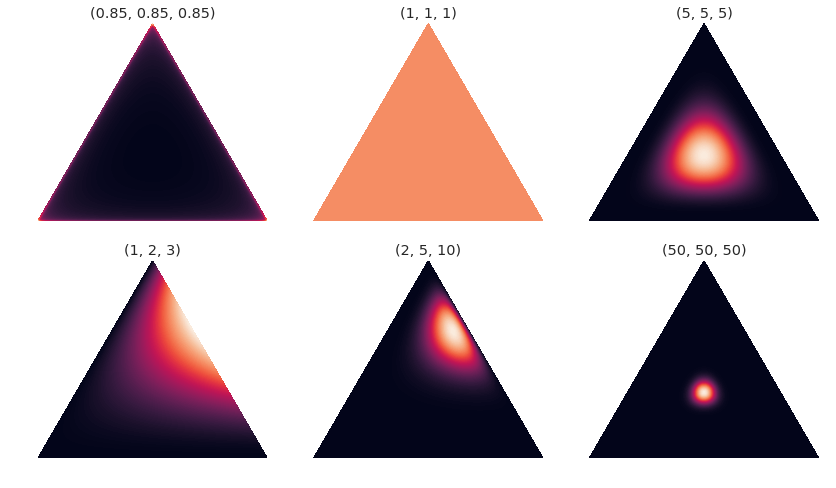
\includegraphics[keepaspectratio=true,scale=0.4]{figuras/dist-diri-simplex.png}
	\caption{Distribuição de $\alpha_1$, $\alpha_2$ e $\alpha_3$ no 2-simplex}
	Fonte: do próprio autor
	\label{fig08}
\end{figure}


Como especificado em \ref{dir:var}, é possível observar que quanto maior o valor de $\alpha_i$, menor a variância na Figura \ref{fig09} que contém um conjunto de cinco distribuições Dirichlet, com $i=10$ e todos os $\alpha$ são iguais. Para cada distribuição a $\sum_{i=1}^{10} \alpha_i = 1$.



\begin{figure}[!h]
	\centering
	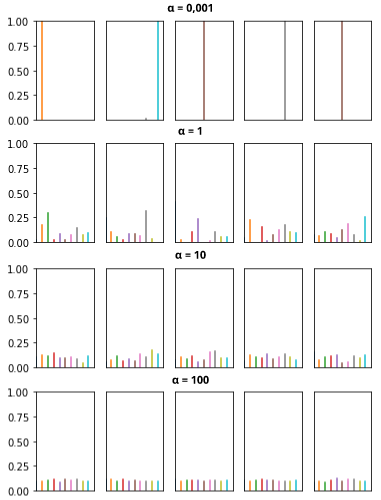
\includegraphics[keepaspectratio=true,scale=0.7]{figuras/dist-diri-var.png}
	\caption{Distribuição Dirichlet com $i=10$ e variações de $\alpha$ = 0,001, 1, 10 e 100 }
	Fonte: do próprio autor
	\label{fig09}
\end{figure}



\section{Processo Bernoulli}

Segundo \cite{bertsekas2008} o processo de Bernoulli pode ser visualizado como uma sequência independente de jogadas de moedas, onde a probabilidade de ser cara em cada jogada é um número fixo p na faixa $0 < p < 1$. Em geral, o processo de Bernoulli consiste em uma sequência de tentativas de Bernoulli, onde cada tentativa produz um 1 (um sucesso) com probabilidade $p$, e um 0 (falha) com probabilidade $1 - p$, independentemente do que acontece em outros ensaios.

Naturalmente, o lançamento de moeda é apenas um paradigma para uma ampla gama de contextos envolvendo uma seqüência de resultados binários independentes. Por exemplo, um processo de Bernoulli é freqüentemente usado para modelar sistemas envolvendo chegadas de clientes ou trabalhos em centros de serviços. O tempo é discretizado em períodos, e um “sucesso” na tentativa $k$ está associado à chegada de pelo menos um cliente no centro de serviços durante o $k$-ésimo período.

Em uma descrição mais formal, é definido o processo de Bernoulli como uma sequência $X1, X2, \dots$ de variáveis aleatórias independentes de Bernoulli $X_{i}$ com

$$P(X_{i} = 1) = \textbf{P}(\textit{sucesso na i-ésima tentativa}) = p $$
$$P(X_{i} = 0) = \textbf{P}(\textit{falha na i-ésima tentativa}) = 1-p $$


para cada $i$. Generalizando a partir do caso de um número finito de variáveis aleatórias, a independência de uma sequência \textit{infinita} de variáveis aleatórias de $X_i$ é definida pela exigência de que as variáveis aleatórias $X1, X2, \dots$ seja independentes para qualquer $n$ finito.


%\subsection{Independência e ausência de memória}
\begin{itemize}
	\item Independência e ausência de memória
\end{itemize}

O pressuposto de independência por trás do processo de Bernoulli tem implicações importantes, incluindo uma propriedade de ausência de memória (o que quer que tenha acontecido em testes anteriores não fornece informações sobre os resultados de ensaios futuros). Uma apreciação e compreensão intuitiva de tais propriedades é muito útil e permite a rápida solução de muitos problemas que seriam difíceis com uma abordagem mais formal.

De acordo com \cite{bertsekas2008} com duas variáveis aleatórias desse tipo e se os dois conjuntos de tentativas que os definem não tiverem um elemento comum, essas variáveis aleatórias serão independentes. Se duas variáveis aleatórias $U$ e $V$ são independentes, então quaisquer duas funções delas, $g(U)$ e $h(V)$, também são independentes.

Supondo que um processo de Bernoulli tenha sido executado por $n$ vezes, e que tenha sido observado os valores experimentais de $X1, X2, ..., Xn$. É notado que a sequência de futuros ensaios $Xn + 1, Xn + 2, ...$ são ensaios independentes de Bernoulli e, portanto, formam um processo de Bernoulli. Além disso, esses testes futuros são independentes dos anteriores. \cite{bertsekas2008} conclui que, a partir de qualquer dado momento, o futuro também é modelado por um processo de Bernoulli, independente do passado. Se faz referência assim, a como a propriede de \textbf{novo início} do processo de Bernoulli.



\section{Aprendizado de Máquina}

Aprendizado de Máquina é uma área de IA cujo objetivo é o desenvolvimento de técnicas computacionais sobre o aprendizado bem como a construção de sistemas capazes de adquirir conhecimento de forma automática. Um sistema de aprendizado é um programa de computador que toma decisões baseado em experiências acumuladas através da solução bem sucedidade de problema anteriories (\cite{Monard2003}). 

\cite{mitchell1997} define que um programa computacional aprende a partir da experiencia E, em relação a uma classe de tarefas T, com medida de desempenho P, se seu desempenho nas tarefas T, medida por P, melhora com a experiência E.


A indução é a forma de inferência lógica que permite obter conclusões genéricas sobre um
conjunto particular de exemplos. Ela é caracterizada como o raciocínio que se origina em um conceito específico e o generaliza, ou seja, da parte para o todo. É um dos principais métodos utilizados para derivar conhecimento novo e predizer eventos futuros. 


O aprendizado indutivo é efetuado a partir de raciocínio sobre exemplos fornecidos por um processo externo ao sistema de aprendizado. O aprendizado indutivo pode ser dividido em supervisionado e não-supervisionado. 


No aprendizado supervisionado é fornecido ao algoritmo de aprendizado, ou indutor, um conjunto de exemplos de treinamento para os quais o rótulo (\textit{label}) da classe associada é conhecido.

Em geral, cada exemplo é descrito por um vetor de valores de características, ou atributos, e o rótulo da classe associada. O objetivo do algoritmo de indução é construir um classificador que possa determinar corretamente a classe de novos exemplos ainda não rotulados, ou seja, exemplos que não tenham o rótulo da classe. Para rótulos de classe discretos, esse problema é conhecido como classificação e para valores contínuos como regressão.

Já no aprendizado não-supervisionado, o indutor analisa os exemplos fornecidos e tenta determinar se alguns deles podem ser agrupados de alguma maneira, formando agrupamentos ou clusters Cheeseman  Stutz 1990. Após a determinação dos agrupamentos, normalmente, é necessária uma análise para determinar o que cada agrupamento significa no contexto do problema que está sendo analisado.


\subsection{Aprendizado Não Supervisionada}
LIVRO: 261

Segundo XXXX, o paradigma da aprendizagem não supervisionada, muitas vezes chamado de agrupamento, envolve um processo que revela automaticamente (descobre) a estrutura dos dados e não envolve nenhuma supervisão. Dado um dataset N-dimensional $X={x_1,x_2,\dots,x_N}$, onde cada $x_k$ é caracterizado por um conjunto de atributos, para identificar e descrever grupos (\textit{clusters}) presente em $X$..


Como o nome \textit{clustering} ou agrupamento implica, espera-se que um algoritmo adequado, não supervisionado, seja capaz de descobrir a estrutura por conta própria explorando semelhanças ou diferenças (como distâncias) entre pontos de dados individuais em um conjunto de dados em consideração. (pg 257) Entretanto, agrupar dois pontos se eles estivem "próximos" ... O número de estratégias diferentes para a formação de \textit{cluster} é enorme, e muitas abordagens tentam determinar qual a "similaridade" entre os elementos nos dados significa. Diferente algoritmos de \textit{clustering} abordam várias facetas e propriedades de clusters..


Técnicas de \textit{clustering} (agrupamento) podem ser divididos em três principais categorias:

- Partição 
- Clustering Hierárquico 
- Model-based (pg 258-262)


\subsection{Aprendizado Supervisionada}

PG: 62


A aprendizagem supervisionada está no outro extremo do espectro de aprendizado não supervisionado na diversidade existente de esquemas de aprendizado. Na aprendizagem não supervisionada, nos são fornecidos dados e solicitados a descobrir sua estrutura.

Na aprendizagem supervisionada, a situação é muito diferente. Recebemos uma coleção de dados (padrões) e sua caracterização, que podem ser expressos na forma de alguns rótulos discretos (caso em que temos um problema de classificação) ou alguns valores de variáveis contínuas auxiliares. Nesse caso, estamos diante de um problema de regressão ou de um problema de aproximação.

Em problemas de classificação, cada ponto de dados $x_k$ vem com um certo rótulo de classe .. "label"


\section{Naive Bayes}

%https://scikit-learn.org/stable/modules/naive_bayes.html

%http://www.cs.unb.ca/~hzhang/publications/FLAIRS04ZhangH.pdf


\section{Análise de Componentes Principais}

OU tb PCA

\section{Latent Dirichlet Allocation}

%http://conteudo.icmc.usp.br/CMS/Arquivos/arquivos_enviados/BIBLIOTECA_158_RT_409.pdf

%http://www.jmlr.org/papers/volume3/blei03a/blei03a.pdf